% Copyright (C) 2014 by Thomas Auzinger <thomas.auzinger@cg.tuwien.ac.at>

\documentclass[draft,final]{vutinfth} % Remove option 'final' to obtain debug information.

% Extended LaTeX functionality is enables by including packages with \usepackage{...}.
\usepackage{fixltx2e}  % Provides fixes for several errors in LaTeX2e.
\usepackage{amsmath}   % Extended typesetting of mathematical expression.
\usepackage{amssymb}   % Provides a multitude of mathematical symbols.
\usepackage{mathtools} % Further extensions of mathematical typesetting.
\usepackage{microtype} % Small-scale typographic enhancements.
\usepackage{enumitem}  % User control over the layout of lists (itemize, enumerate, description).
\usepackage{multirow}  % Allows table elements to span several rows.
\usepackage{booktabs}  % Improves the typesettings of tables.
\usepackage[ruled,linesnumbered,algochapter]{algorithm2e} % Enables the writing of pseudo code.
\usepackage{nag}       % Issues warnings when best practices in writing LaTeX documents are violated.
\usepackage{hyperref}  % Enables cross linking in the electronic document version. This package has to be included second to last.
\usepackage[acronym,toc]{glossaries} % Enables the generation of glossaries and lists fo acronyms. This package has to be included last.

\usepackage{placeins}

\setsecnumdepth{subsection} % enumerate subsections

% Use an optional index
\makeindex
% Use an optional glossary
\makeglossaries
%\glstocfalse % remove the glossaries from the table of contents

% Set persons with 4 arguments:
%  {title before name}{name}{title after name}{gender}
%  where both titles are optional (i.e. can be given as empty brackets {})
\setauthor{}{Patrick Bellositz}{}{male}
\setadvisor{Ao.Prof.Dipl.-Ing.Dr.techn.}{Christian Georg Ferm{\"u}ller}{}{male}

% For dissertations
\setfirstreviewer{Pretitle}{Forename Surname}{Posttitle}{male}
\setsecondreviewer{Pretitle}{Forename Surname}{Posttitle}{male}

% Required data
\setaddress{Address}
\setregnumber{1027108}
\setdate{01}{01}{2001}
\settitle{Abstract Argumentation Frameworks}{Abstract Argumentation Frameworks} % sets English and German version of the title (both can be English or German)

\setthesis{bachelor}

% For bachelor and master
\setcurriculum{Software \& Information Engineering}{Software \& Information Engineering} % sets the English and German name of the curriculum

\begin{document}

\frontmatter % switches to roman numbering
% The structure of the thesis has to conform to
%  http://www.informatik.tuwien.ac.at/dekanat

%\addtitlepage{naustrian}
\addtitlepage{english} % English title page
\addstatementpage

\begin{danksagung*}
Ihr Text hier.
\end{danksagung*}

\begin{acknowledgements*}
Enter your text here.
\end{acknowledgements*}

\begin{kurzfassung}
Ihr Text hier.
\end{kurzfassung}

\begin{abstract}
Enter your text here.
\end{abstract}

% Select the language of the thesis, e.g., english or naustrian.
\selectlanguage{english}

% Add a table of contents (toc)
\tableofcontents % starred version, i.e., \tableofcontents*, removes the self-entry

% Use an optional list of figures
\listoffigures % starred version, i.e., \listoffigures*, removes the toc entry

% Use an optional list of tables
\listoftables % starred version, i.e., \listoftables*, removes the toc entry

% Use an optional list of alogrithms
\listofalgorithms
\addcontentsline{toc}{chapter}{List of Algorithms}

% Switch to arabic numbering and start the enumeration of chapters in the table of content.
\mainmatter

\chapter{Introduction}
Enter your text here.

\chapter{Additional Chapter}
test
	\begin{figure}[!htb]
		\centering
		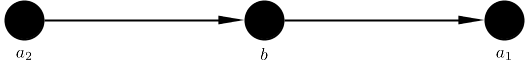
\includegraphics[width=\linewidth]{graphics/ex1.png}
		\caption{An argument framework about colors.}
	\end{figure}
test

\backmatter

% Add a bibliography
\bibliographystyle{alpha}
\bibliography{intro}

% Add an index
\printindex

% Add a glossary
\printglossaries



\end{document}